\chapter{RC and RL Transient Signals}

\section{Introduction}

In this lab you will use explore transient behavior of $RC$ and $RL$
circuits.  You will learn how to configure the trigger of your digital
oscilloscope.  You will learn how to use scope probes and measure
properties of waveforms on your digital oscilloscope using cursors.
For this lab there are both logbook and Jupyter notebook entries.

\section{Oscilloscope Trigger}

This section introduces the trigger feature of your digital
oscilloscope.  It should not take more than about one half hour.

\begin{figure}[htbp]
\begin{center}
\begin{tabular}{cc}
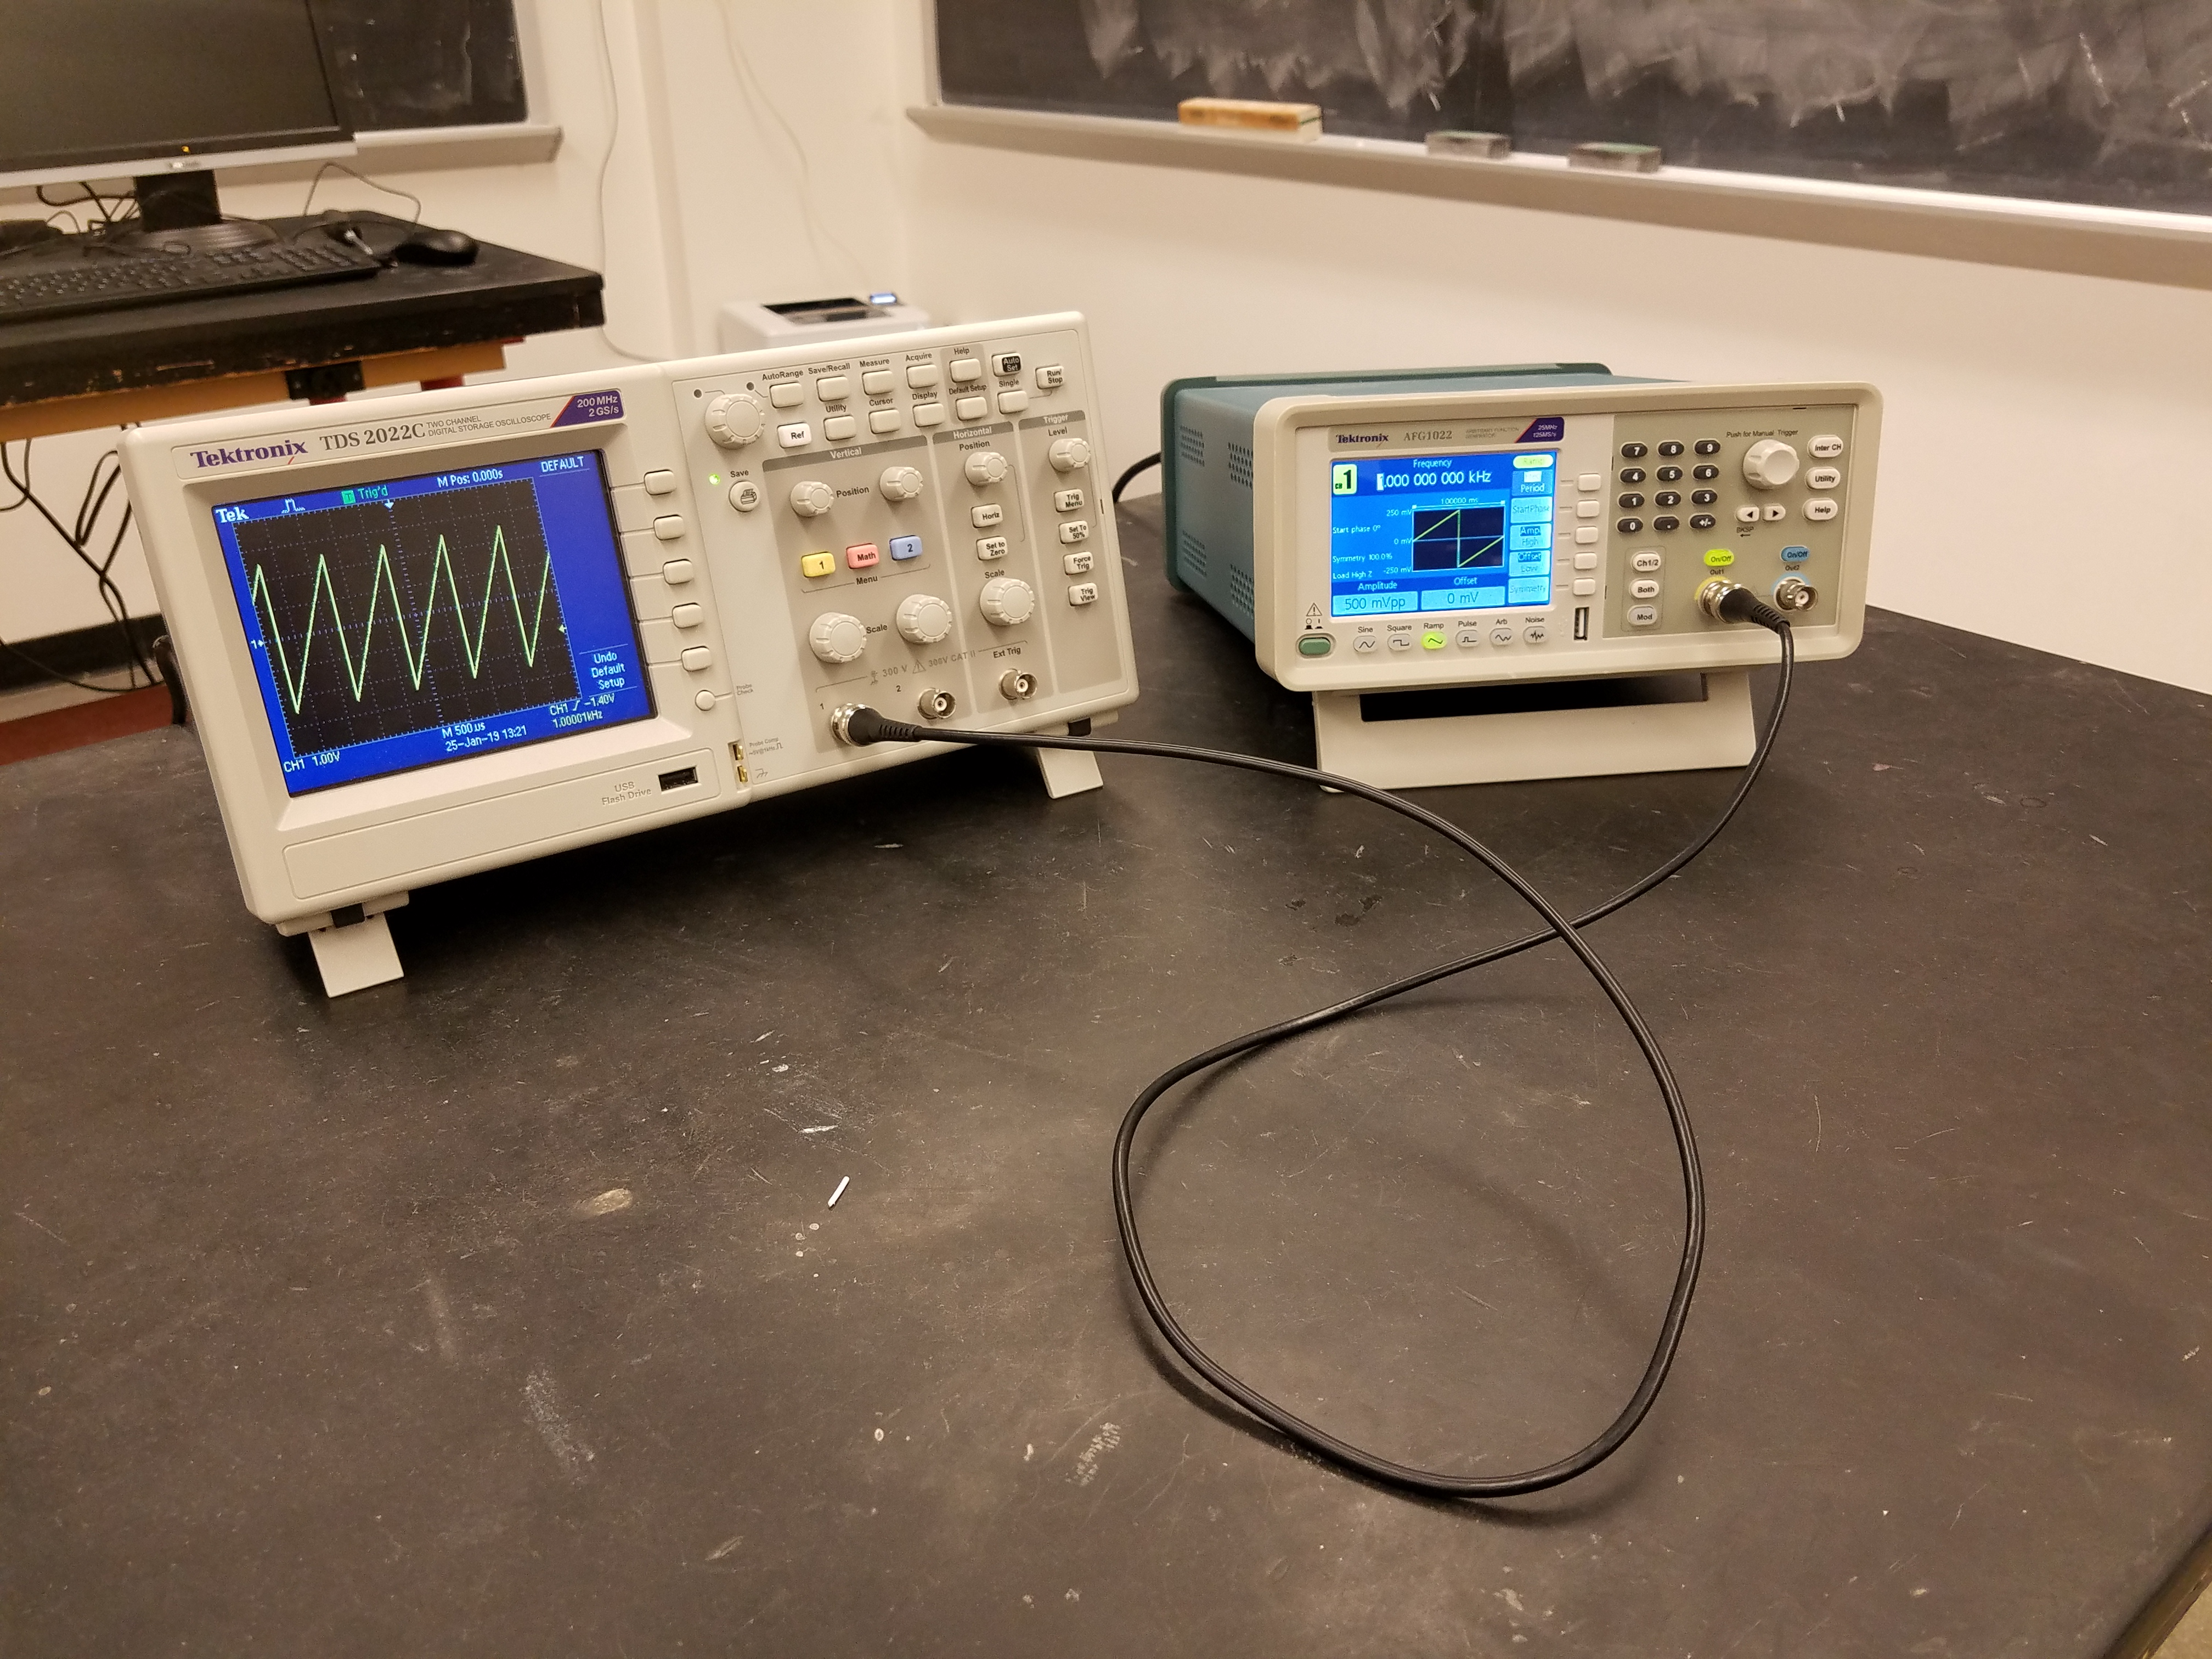
\includegraphics[width=0.40\textwidth]{figs/labs/transients/ramp_setup.jpg}  &
\begin{tikzpicture}
    \node[anchor=south west,inner sep=0] (image) at (0,0,0) {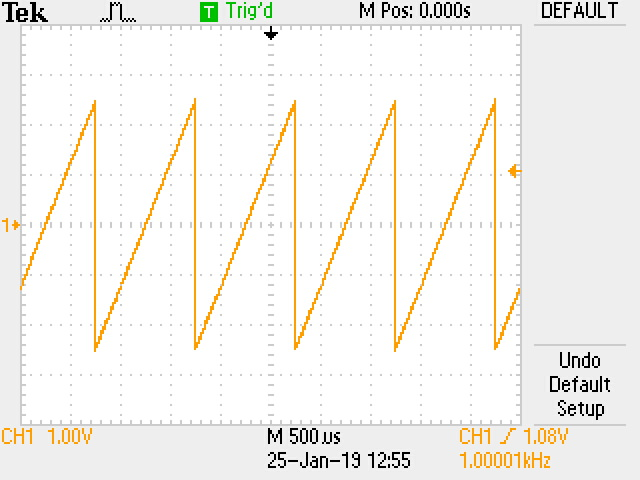
\includegraphics[height=0.25\textheight]{figs/labs/transients/trigger_ramp.jpg}};
    \node[left](X) at (0,5.3) {$t=0$};
    \draw (X.east) -- (3.3,5.7);
    \node[right](X) at (8.0,5.0) {\parbox{1cm}{Trigger \\ Threshold}};
    \draw (X.west) -- (6.5,3.9);
\end{tikzpicture}\\
(a) & (b) \\
\end{tabular}
\caption{(a) Setup for the scope trigger measurement, and (b) A scope trace triggered by the rising edge of ramp function.  The point $t=0$ is the location where the waveform first crosses the trigger thresholds, which is indicated by the arrow to the right.}
\label{fig:ramp_setup}
\end{center}
\end{figure}

Connect the output of Channel 1 on your function generator directly to
Channel 1 of your oscilloscope with a BNC cable, as in
Fig.~\ref{fig:ramp_setup}a.  Set your function generator to produce a
$1~\rm kHz$ Ramp function with a peak-to-peak amplitude of $600~\rm
mV$. While the Ramp function is selected, you will have an option
``Symmetry'' available.  Press the menu button next to Symmetry and
set the value to 100\%.  Recall that you need to remember to (1) set
your function generator to expect high-impedance output, (2) enable
the function generator output by pressing the ``On/Off'' button above
the BNC connector for the channel, so that button is lit (this is the
last time these steps will be explicitly mentioned.)

Turn on your oscilloscope and press the ``Default Setup'' button.  The
ramp function should be immediately visible on your scope.  Adjust the
attenuation factor of Channel 1 to unity (X1) appropriate for BNC
cable and confirm the peak to peak amplitude and the period are as
expected (Leave Channel 2 alone for now.)

Your scope is continuously updating the display with the most recently
collected waveform, which at $1~\rm kHz$ is effectively instantaneous.
You may have wondered how these images all appear on the oscilloscope
with the exact same phase.  This crucial feature of your scope is a
result of its trigger feature, which we'll explore now.  Turn the knob
labeled ``Trigger Level'' and you should see the phase of your
waveform change. Notice that the trigger value and trigger type is
displayed, and that the trigger value changes as your turn the knob.

As shown in Fig.~\ref{fig:ramp_setup}b, your scope display has an arrow at
the top of the display which indicates the point at which the trigger
condition was met for the current waveform, which is taken as $t=0$.
A second arrow, along the right side, indicates the trigger threshold.
Your scope is configured to trigger on the rising edge, which means it
will trigger at the instant where the trigger first goes above the
trigger threshold.

As you adjust the trigger threshold, the point at which the waveform
reaches this threshold changes.  Since $t=0$ is defined by the instant
at which the trigger condition is met, this effectively changes the
phase of your waveform.  As you adjust the threshold up and down, the
waveform moves forward and backward along the time axis.  This is an
example of an effect called ``time-slewing'', which is important to
consider when making time dependent measurements of wave forms, as we
will be doing today.

Notice what happens if you dial the threshold until it exceeds the
amplitude of your waveform.  Suddenly, your waveform will appear to
dance across the screen.  This is because your scope trigger is set to
``Auto'' trigger.  In this trigger mode, when too much time has passed
without the trigger condition being met, a waveform is displayed for
the current input using a random time for $t=0$.  This can be
convenient for finding a signal of unknown size and location.

Press the ``Trigger Menu'' button, and then set the Trigger Mode to
``Normal'' by pressing the corresponding menu button.  In this Mode,
the waveform is not updated until a trigger is received.  While the
scope is in the Normal trigger mode, adjust the threshold so that it
is above the amplitude of the waveform.  You will notice that when the
trigger condition is not being met, the scope indicates the state
``Ready'' at the top of the screen, meaning that the scope is armed to
collect data when the trigger condition is met, but there has not
recently been a trigger.  Now move the threshold below the amplitude
for the waveform, and you should see the scope indicates the state
``Trig'd'', or triggered, on this display.  A common mistake for
students is to look at stale data, without realizing that the signal
is lost.  Avoiding this pitfall is one benefit of the Auto trigger
mode.

At times you may wish to start and stop the data acquisition.  This
can be accomplished using the ``Run/Stop'' button to pause and then
resume waveform acquisition.  Try this feature out now.  You can also
capture and display one single wave form by pressing the ``Single
Seq'' button.  This can be handy when looking at things like detector
pulses, which are different each time, and which may occur at a low
rate.  Resume normal data acquisition with the ``Run/Stop'' button.

Your scope trigger has the capability of triggering on either the
rising edge or the falling edge of the input.  When triggering on the
rising edge, the trigger fires at the instant the waveform first
exceeds the trigger threshold.  When triggering on the falling edge,
the trigger fires at the instant the waveform first falls below the
trigger threshold.  Using the appropriate menu button, set your scope
to trigger on the ``Falling'' edge.  You should observe that now the
$t=0$ occurs at the nearly straight vertical line in our ramp
function.  You'll also notice that adjusting the trigger threshold now
has no discernible effect on the phase of the waveform.  Triggering on
sharp edges eliminates the effect of time-slewing, a fact we will
exploit to make accurate time measurements.

\begin{plot}
Save a scope trace obtained while triggering on the falling edge of the ramp function.
\end{plot}

\section{Transient Response of an $RC$ Circuit}

Set Channel 1 of your function generator to produce Square wave output
with a peak-to-peak voltage of $6~\rm V$ and a frequency of $1~\rm
kHz$.  As shown in Fig.~\ref{fig:probe_setup}, use a BNC Tee adapter
to split your signal into two identical outputs.  Send output of the
tee directly to Channel 1 of your scope.  Send the other copy to a
BNC-alligator-pair cable.

\begin{figure}[htbp]
\begin{center}
\begin{tikzpicture}
    \node[anchor=south west,inner sep=0] (image) at (0,0,0)
         {\includegraphics[height=0.30\textheight]{figs/labs/transients/probe_setup.jpg}};
         \node[left](X) at (-1.0,4.0) {Probe Tip}; \draw (X.east) --
         (5.0,2.4); \node[left](X) at (-1.0,3.0) {Ground Clip}; \draw
         (X.east) -- (5.4,2.2); \node[right](X) at (10.0,5.0) {BNC
           Tee}; \draw (X.west) -- (8.0,5.2); \node[right](X) at
         (10.0,4.0) {Alligator pair}; \draw (X.west) -- (6.5,2.8);
\end{tikzpicture}
\caption{A setup for connecting the scope probe directly to the output of the function generator.}
\label{fig:probe_setup}
\end{center}
\end{figure}

Install an oscilloscope probe at Channel 2 of your scope (see
Fig~\ref{fig:probe}).  Some probes in the lab have the ability to
switch between attenuation factors near the probe tip.  If you have
such a probe, select the 10X setting.  The remaining probes have a
fixed attenuation of 10X.

So far, we haven't had to worry about proper grounding procedure,
because this is automatically handled by the BNC cable.  Your scope
probe has two main parts, the larger probe tip, which slides to reveal
a hook which can be attached to wires and components in your circuit,
and a short lead ending with a black alligator clip called the
``Grounding clip''.  Handheld devices like your DMM have no connection
to earth ground.  The voltage reference point at the Common terminal
can be connected anywhere you would like in a circuit.  Your scope is
quite different!  It plugs into a wall outlet for power and is
referenced to earth ground.  To provide a scope which is both safe and
cost effective, most scopes are limited to making measurements which
are referenced to ground when using ordinary probes.  The ground clip
of your scope can only be connected to earth ground.  If you connect
it anywhere else in your circuit, that part of your circuit will be
short-circuited to ground.

For now, connect the probe directly to the output of the function
generator.  Your function generator is also referenced to earth
ground.  In particular for this setup, the black alligator clip is
earth ground.  Connect the black clip from the function generator to
the grounding clip for the scope probe.  Next connect the scope probe
to the red alligator clip from the function generator.  You now have
two copies of the function generator output being sent to the scope.
One directly through the BNC cable, and one through a 10X attenuation
scope probe.

Adjust your scope to view the function generator output as measured by
Trigger 1.  Set the voltage scale as large as possible while observing
the entire wave form.  Leave the timescale at the default setting of
$500~\mu s$ for now.  Check that trigger is on the Falling edge, as set
in the last section.  Set the trigger threshold near 0 volts.
You should observe that the position of the waveform does not vary
much with trigger threshold: the steep falling edge of the square wave
function gives us a solid reference point for defining $t=0$ in the
measurements that follow.

Now enable Channel 2 on your scope. Adjust all the necessary settings
for Channel 2 so that it produces an identical copy of Channel 1.  Too
see both channels at the same time, you'll have to move the vertical
position of Channel 1 slightly.  Closed loop tests like this are the
way experienced scientists and engineers always start.  It allows you
to setup your signal generator and scope properly, without adding the
complexity of the circuit you are working on.  In general, avoiding
confusion by taking small incremental steps is the fastest, most
reliable way to proceed in lab.

\begin{figure}[htbp]
\begin{center}
\begin{tabular}{cc}
\begin{circuitikz}[line width=1pt]
\draw (0,0) to[square voltage source,bipoles/length=1.5cm] ++(0,4.0) to[short] ++(2.0,0)
to[R,-*] ++(0,-2.0) coordinate(X) to[short,*-o] ++(1.0,0) node[right]{A};
\draw (X) to[C,-*] ++(0,-2.0) coordinate(X) to[short,-o] ++(1.0,0) node[right]{B};
\draw (X) to[short,-*] ++(-2.0,0) node[ground,yscale=2.0]{};
\end{circuitikz}  &
\begin{circuitikz}[line width=1pt]
\draw (0,0) to[square voltage source,bipoles/length=1.5cm] ++(0,4.0) to[short] ++(2.0,0)
to[R,-*] ++(0,-2.0) coordinate(X) to[short,*-o] ++(1.0,0) node[right]{A};
\draw (X) to[L,-*] ++(0,-2.0) coordinate(X) to[short,-o] ++(1.0,0) node[right]{B};
\draw (X) to[short,-*] ++(-2.0,0) node[ground,yscale=2.0]{};
\end{circuitikz}  \\
(a) & (b) \\
\end{tabular}
\caption{A function generator driving an (a) RC circuit, and (b) RL circuit.}
\label{fig:rlc-circuits}
\end{center}
\end{figure}

Select a $C=10~\rm nF$ capacitor and an $R=10~\rm k\Omega$.

\begin{measurement}
Using the given values of resistor and capacitor, calculate and record
in your logbook the time constant of the RC circuit.  Using your DMM,
measure and record the actual resistance and capacitance of your
components before installing them.
\end{measurement}

Construct the circuit in Fig.~\ref{fig:rlc-circuits}a on your
breadboard, as shown in Fig.~\ref{fig:rc_setup}a.  Your function
generator acts as the square wave voltage source.  Recall that the
black alligator clip is earth ground.  The red alligator clip is the
square wave output relative to earth ground, and corresponds to the
upper terminal of the voltage source in the diagram.  The only valid
place to connect the grounding clip of your scope probe is to earth
ground, so connect that to point B in your circuit.  Connect the scope
probe tip to point A.  As shown in the Fig.~\ref{fig:rc_setup}b, each
time the square wave changes polarity, the capacitor begins charging
or discharging until it reaches equilibrium with the new voltage,
revealing the characteristic exponential transient response.

\begin{figure}[htbp]
\begin{center}
\begin{tabular}{cc}
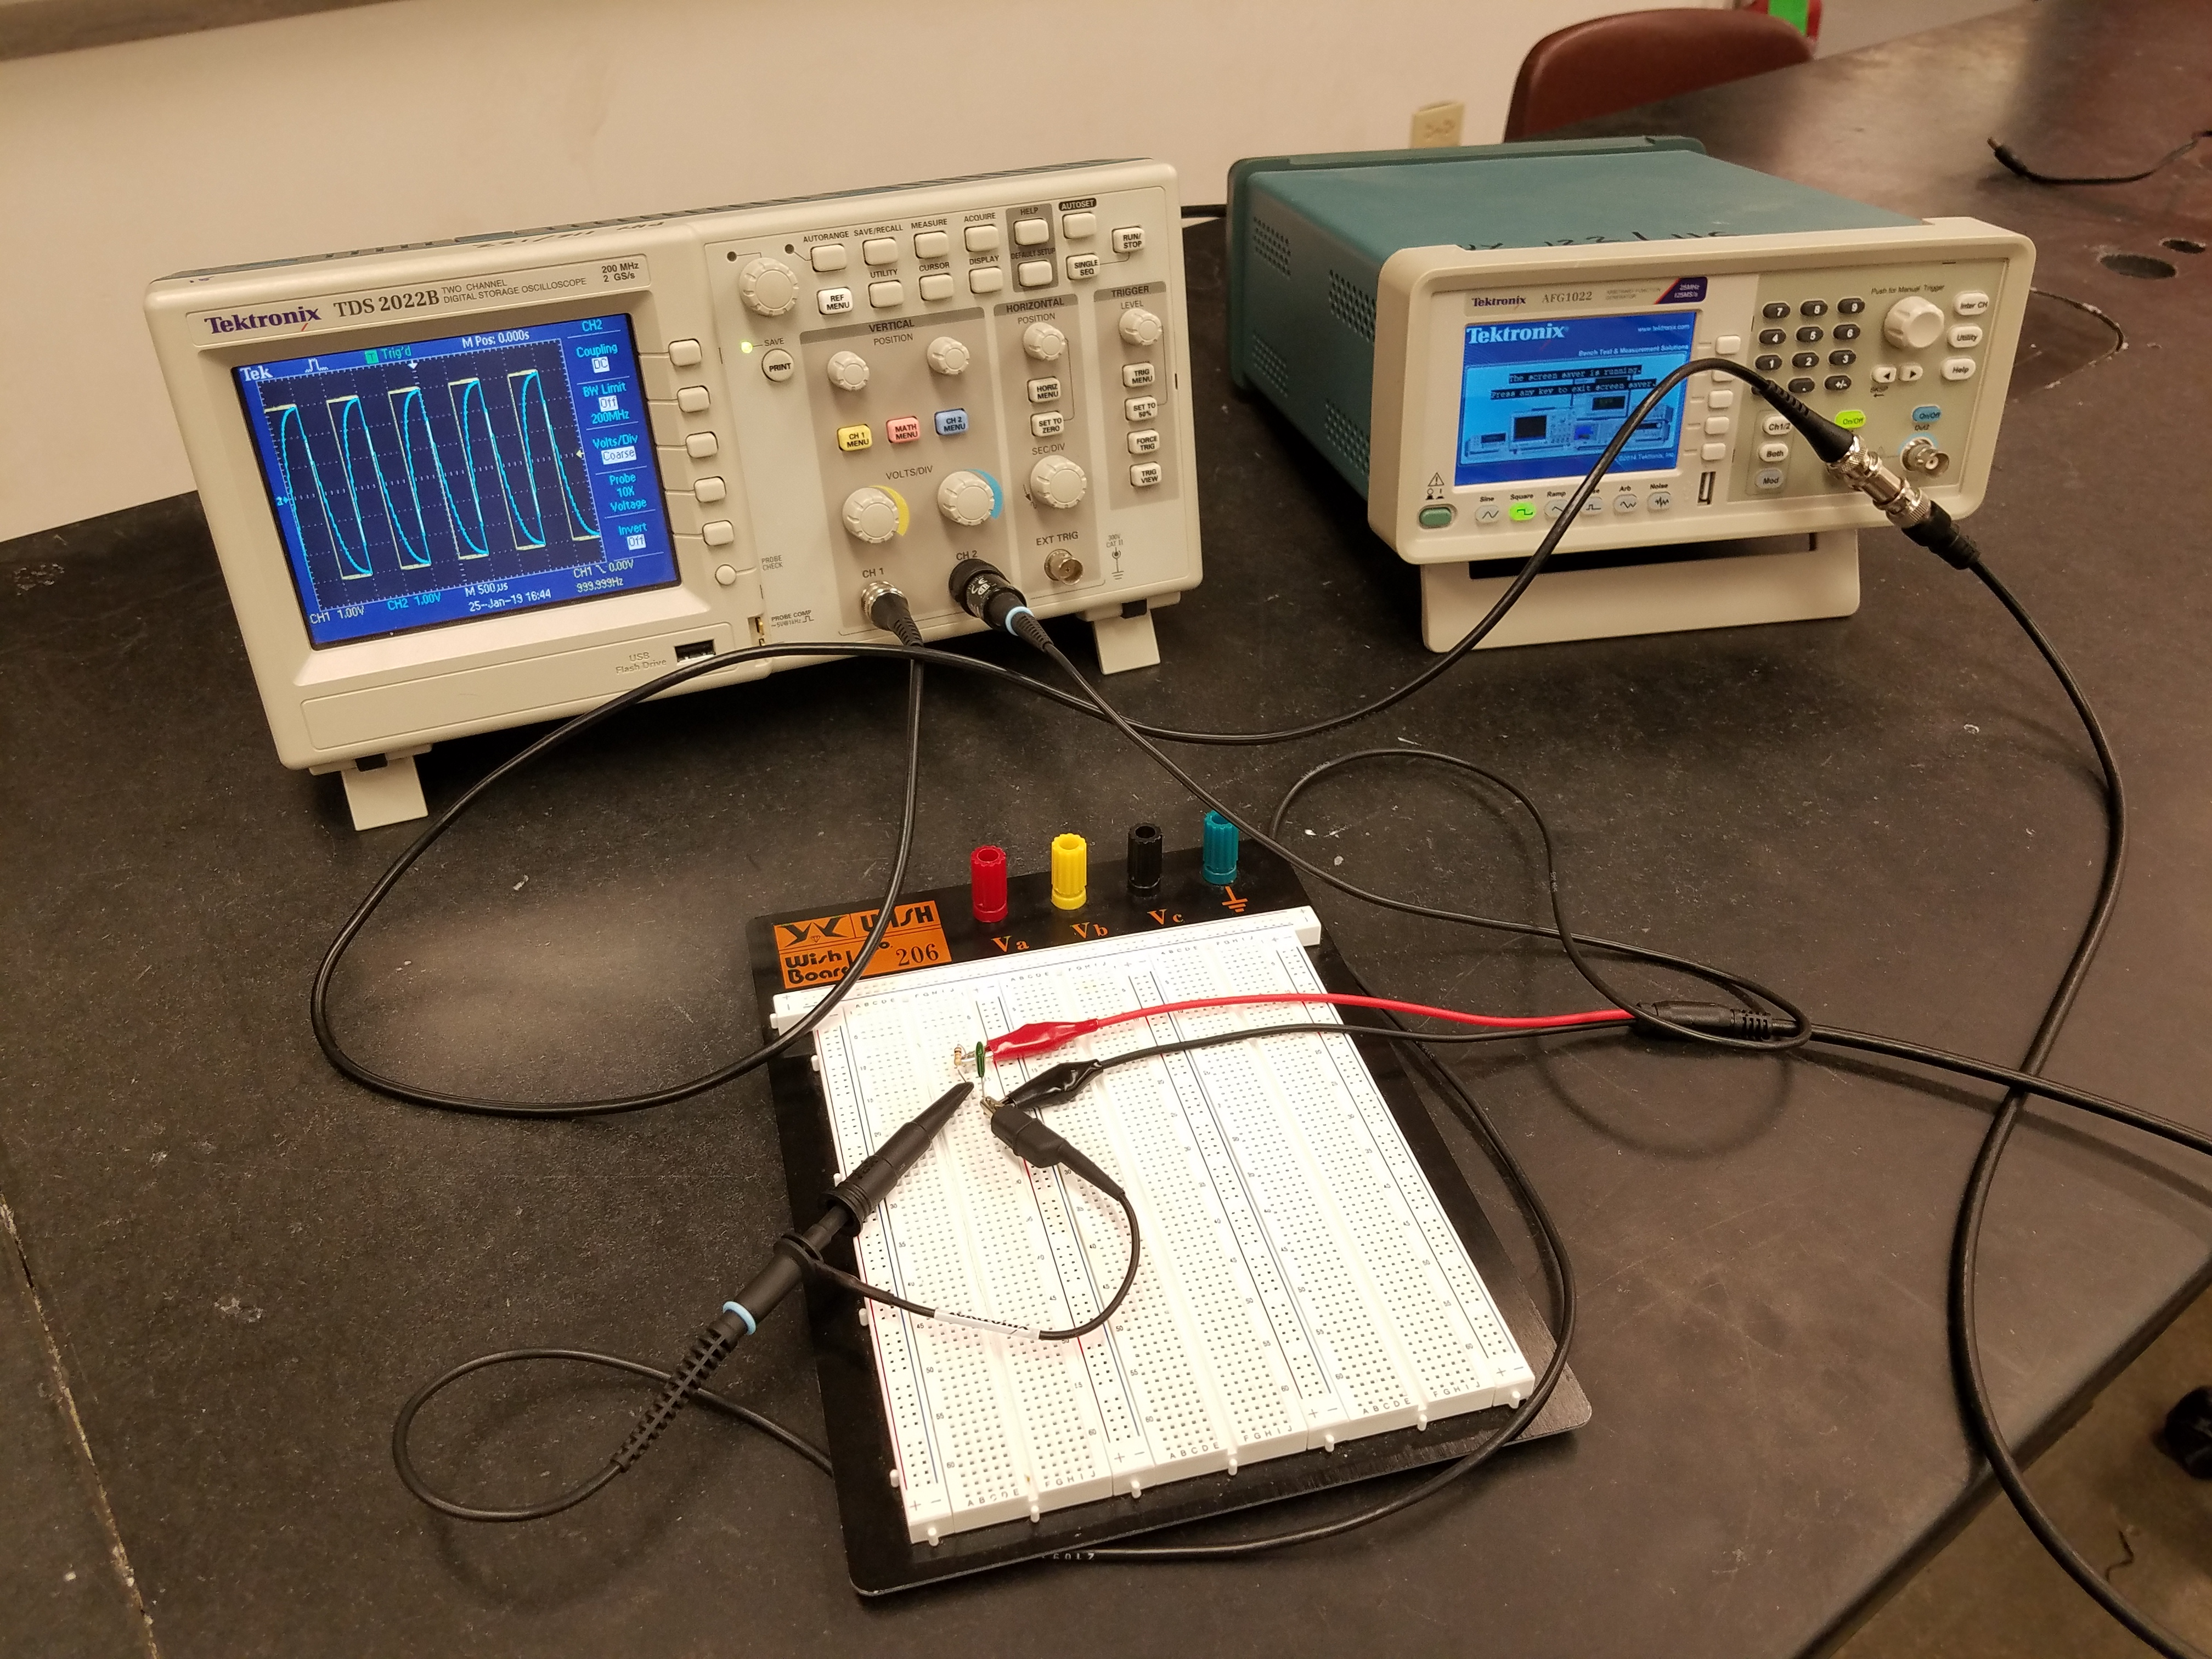
\includegraphics[width=0.45\textwidth]{figs/labs/transients/rc_setup.jpg} &
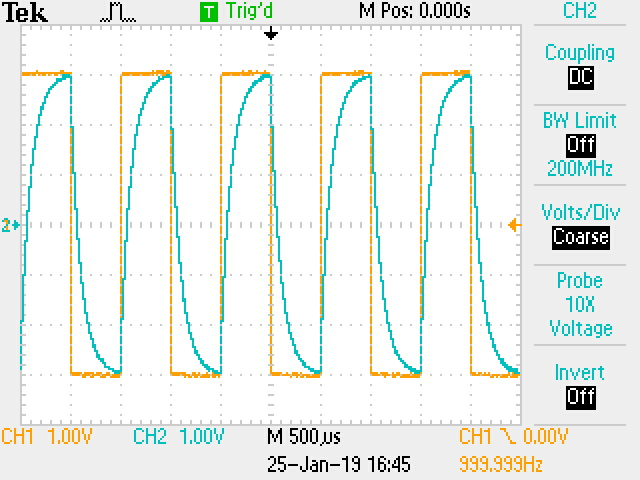
\includegraphics[width=0.45\textwidth]{figs/labs/transients/rc_trace.jpg} \\
(a) & (b) \\
\end{tabular}
\caption{Setup for the (a) RC circuit measurement, and (b) example scope trace showing exponential curve.}
\label{fig:rc_setup}
\end{center}
\end{figure}

\begin{figure}[htbp]
\begin{center}
\begin{tabular}{cc}
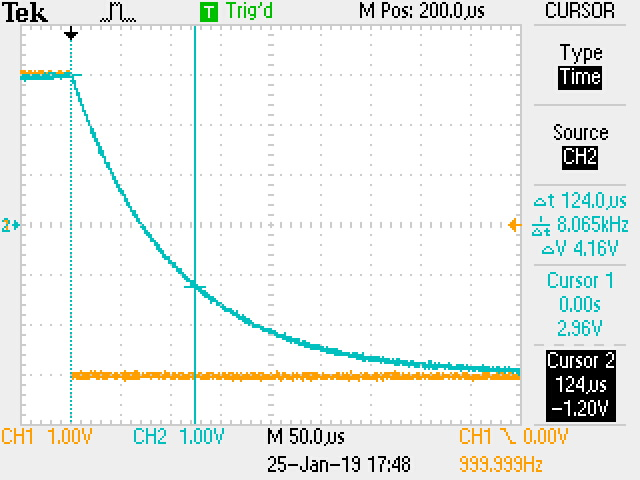
\includegraphics[width=0.45\textwidth]{figs/labs/transients/rc_cursor.jpg} &
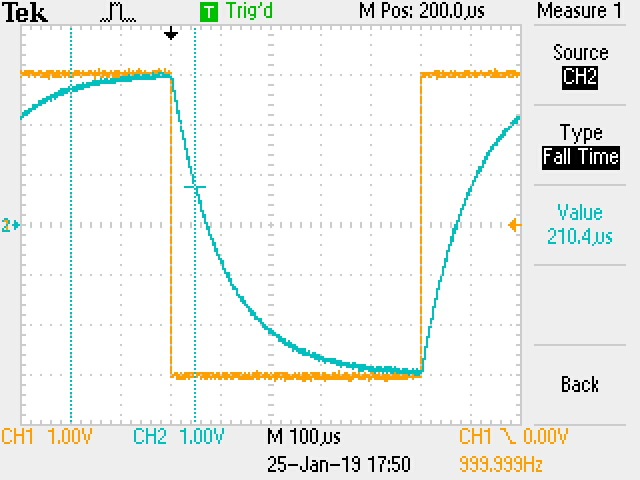
\includegraphics[width=0.45\textwidth]{figs/labs/transients/rc_falltime.jpg} \\
(a) & (b) \\
\end{tabular}
\caption{Scope traces showing (a) use of cursor to measure the waveform at $t=124~\rm \mu s$ and $V=-1.20~\rm V$, (b) use of the built in fall time measurement.}
\label{fig:cursor_falltime}
\end{center}
\end{figure}

Now adjust the timescale to zoom in on the exponential decay portion
of the curve, making sure to keep the trigger position at the left
side of the display, as shown in Fig.~\ref{fig:cursor_falltime}a.
Press the Cursor button, then set Type to Time, and Source to CH2.
This feature allows you to make measurements of different points along
the curve.  Leave Cursor 1 located at $t=0$.  Highlight Cursor 2, by
pressing the corresponding menu button, and adjust it's position using
the multipurpose knob.  Now you can make accurate measurements of the
waveform by reading off the voltage and time at anywhere that you
place the cursor.  

\begin{measurement}
Record one measurement every $\sim 25~\rm \mu s$ starting from
$t=0~\mu s$ to $400~\rm \mu s$.  (Recall that when making measurements
at target values, you need not hit the target value exactly, simply
record the actual position at which you made your measurement.) Record
a rough sketch of your waveform.
\end{measurement}

For an exponential decay with time constant $\tau$, the rise-time (or fall-time),
when defined as the time interval between $10\%$ and $90\%$ values, is
given by:
\begin{displaymath}
t_{90} = {\rm ln}(9) \; \tau \sim 2.2 \; \tau
\end{displaymath}

\begin{measurement}
Your scope can also directly measure the fall time of a waveform.  For
an accurate measurement, setup the scope so that one complete falling
edge is on screen, as shown in Fig.~\ref{fig:cursor_falltime}b.  Press
Measure and then set source to CH2 and Type to ``Fall Time''. You
might see this value fluctuating.  In such circumstances, it's a good
practice to record 3-5 different measurements to help intepret your
results later.

The manufacturer does not specify the accuracy of the fall-time
measurement, but from other specifications we can reasonably infer an
accuracy of about $3\%$ for the setting used in this lab.  The values of $R$ and $C$ measured with your DMM are much more precisely known than $3\%$.  Does your predicted time-constant based on the measured values of $R$ and $C$ agree with the measured fall time?
\end{measurement}

This is a \textbf{sign-off point} for this lab.

\begin{plot}
Plot your collected $RC$ circuit voltage-versus-time data as discrete
data points.  On the same plot, compare the data to the expected
exponential decay function as a continuous curve, using the $RC$ time
constant calculated from the measured values of $R$ and $C$.  Make
sure to have appropriate axis labels and a legend indicating ``Data''
and ``Prediction''.
\end{plot}
  
\section{Transient response of an RL circuit}

Not everyone will have time to finish this entire section, do your
best with your available time.

\begin{measurement}
Calculate the inductance of a solenoid with N=20 turns, length
$\ell=4~\rm cm$, a radius of $1~\rm cm^2$ using the formula:
\begin{displaymath}
L = \frac{\mu_0 N^2 A}{\ell}
\end{displaymath}
where $A$ is the cross-sectional area and $\mu_0 = 1.257 \times 10^{-6}~\rm H/m$.
\end{measurement}

\begin{measurement}
Wrap an inductor around the provided wooden dowel. Estimate it's
inductance by modifying your calculation above accordingly and record
the value in your logbook.
\end{measurement}

Obtain a $R=47~\rm \Omega$ resistor.
\begin{measurement}
Using your DMM, measure and record the resistance of your resistor.
\end{measurement}

Turn down the supply to $2.5~\rm V$ peak-to-peak.  Build the
circuit in Fig.~\ref{fig:rlc-circuits}b using your homemade inductor
and your resistor.

\begin{measurement}
Using your digital scope, measure the fall-time of your RL circuit and
use it to determine a measured value for the inductance.  Calculate
the inductance of your coil homemade coil and compare to your
theoretical estimate.  Briefly explain your result in your logbook
\end{measurement}

This is an additional \textbf{sign-off point} for this lab.
